
\documentclass[journal]{IEEEtran}
\usepackage{url}
\usepackage{listings}
\usepackage{subfig}
\hyphenation{op-tical net-works semi-conduc-tor}
\usepackage{courier}
\usepackage{xcolor}
\usepackage{graphicx}
\usepackage{hyperref}
\usepackage{array}
\usepackage{pdfpages}


\setlength{\parskip}{\baselineskip}%
\setlength{\parindent}{0pt}%
\definecolor{dkgreen}{rgb}{0,0.6,0}
\definecolor{gray}{rgb}{0.5,0.5,0.5}


%\setmonofont{Consolas} %to be used with XeLaTeX or LuaLaTeX
\definecolor{keyw}{HTML}{BB94B2}
\definecolor{cmmt}{HTML}{969896}
\definecolor{str}{HTML}{68BDB5}
\definecolor{types}{HTML}{74C6F0}
\definecolor{linenr}{HTML}{999999}
%\definecolor{bg}{HTML}{1D1F21}
\definecolor{bg}{HTML}{FFFFFF}
%\definecolor{basic}{HTML}{C6C8C5}
\definecolor{basic}{HTML}{1D1F21}
\setlength\extrarowheight{5pt}
\renewcommand{\arraystretch}{1.3}

\lstset{language=[Sharp]C,
captionpos=b,
numbers=left, %Nummerierung
numberstyle=\ttfamily\tiny\color{linenr}, % kleine Zeilennummer
numbersep=5pt,
keepspaces=true,
tabsize=2,
frame=lines, % Oberhalb und unterhalb des Listings ist eine Linie
showspaces=false,
showtabs=false,
breaklines=true,
showstringspaces=false,
breakatwhitespace=true,
escapeinside={(*@}{@*)},
commentstyle=\color{cmmt},
morekeywords={partial, var, value, get, set, foreach, in, =, +, -, *, /},
keywordstyle=\color{keyw},
stringstyle=\color{str},
backgroundcolor=\color{bg},
basicstyle=\ttfamily\small\color{basic},
}

\lstdefinestyle{inline}{language=[Sharp]C,
  breaklines=true,
  escapeinside={(*@}{@*)},
  commentstyle=\color{cmmt},
  morekeywords={partial, var, value, get, set, foreach, in, =, +, -, *, /},
  keywordstyle=\color{keyw},
  basicstyle=\ttfamily\small\color{basic}
}

\begin{document}
\title{Presentation API Implementation}

\author{Lukas~Tetzlaff,~Nico~Tasche,~Simone~Egger\\Advisor: Louay~Bassbouss}
\markboth{PJ Advanced Web Technologies WS16/17}
{Fraunhofer Fokus FAME, TU Berlin}\maketitle
\section{Abstract}
\label{abstract}
The scope of this document is set to report details about the implementation of the World Wide Web Consortium's Presentation API. The specification was published by the Second Screen Presentation Working Group and submitted as a Candidate Recommendation in July 2016 with the current Editor's Draft version being dated to February, 16 2017.

Paraphrased, the API aims to provide a generalized way of accessing and connecting display resources using web technology thus providing means to present content from a given website to a display and gain restricted remote access to their browsing context by messaging. Effectively this system relies on two dedicated roles, the Controller and the Receiver, obtained by the respective User Agents of on the one hand the initiating web page and on the other hand the display, whereas these may also be identical thus allowing a 1-User-Agent situation. This document and the implementation assume the  2-User-Agent case since 1-UA is to be most prominently used in conjunction with a native way of transmitting the rendered presentation for example by encoding to png and sending it to an external display entity.
\section{Architecture}
\label{architecture}
To facilitate using the Presentation API in terms of hosting a presentation, connecting to a presentation and using the established connection the interface to the user or rather the application developer is kept simple and straight-forward as to be seen in the  \ref{demo}. Generally speaking there are three distinct entities involved in the aforementioned processes, the first being the Receiving User Agent. In case of a browser vendor's implementation of the API this is most likely to be integrated into the browser natively or as a plugin, whereas in this implementation it's a polyfill housed in a loaded html-document, hereafter referred to as the *Receiver*.

The counterpart is the Controlling Browser Agent which acts upon input from the controlling browsing context. Due to the closely coupled relation in the internal procedures of the specification those two entities have been combined into the *Controller* which can be any regular web page enriched by the same aforementioned PresentationAPI-polyfill and scripts containing the desired controller logic of the application developer.

As soon as the Controller knows about the possibility to present on a remote display (Presentation Availability) it may start a Presentation Connection and instruct the Receiver to create a receiving browsing context, here referred to as the *Presentation*, which is the final third component. This is another document written by the application developer that needn't be much different from the regular controlling page since it can identify if it is loaded as a Presentation and act accordingly.

Since the specification relies heavily on individual vendor-specific mechanisms this implementation also provides a configuration interface for the User Agent level that requires a set of handlers \ref{configuration}. To prove this concept two distinct approaches were realized, as seen in  \ref{demo}, one relying purely on ajax and long-polling thus offering maximum compatibility and the second one on WebSockets for a more standard bidirectional low-latency communication, abstracted by third-party library SocketIO which by default also includes a long-polling fallback.

As of this implementation the required logic was split up in separate files that need to be included as seen below.
\subsection{Scripts}
\label{scripts}
In the following table  {\lstinline[style=inline]$C$} denotes the Controller,  {\lstinline[style=inline]$R$} the Receiver and  {\lstinline[style=inline]$RC$} the Receiving Context.

\begin{table}[!ht]\caption{Scripts}\label{scripts}
\centering\begin{tabular}{|l|c|c|c|l|}
\hline 
Script & C & R & RC & Description\\
\hline 
util.js & Y & Y & Y & General utilities to stay vanilla\\
\hline 
presentation.js & Y & Y & Y & Polyfill of Presentation API\\
\hline 
presentationUserAgent.js & Y & Y &  & Vendor-specific realization\\
\hline 
implementation.*.js & Y & Y &  & Implementation-specifics\\
\hline 
receiver.js &  & Y &  & Hosting once loaded / Backdrop\\
\hline 
receivingContext.js &  &  & Y & Communication with R-UA\\
\hline 
*.js &  &  &  & Client scripts that use the API\\
\hline 
\end{tabular} 
\end{table}



Each entity in a Presentation scenario includes the API Polyfill, whereas only Controller and Receiver include the tasks the User Agent shall fulfill globally or in the background to provide relative safety to the receiving context thus preventing it to be conquered by malicious Controllers and displaying content that's not intend to be presented (think of a game without a fixed set of commands in which a Controller was able to inject code to manipulate player's scores or similar situations).
\subsection{Configuration}
\label{configuration}
Every User Agent has a set of handlers that are to be configured apart from the - generally speaking - browser vendor specific functionality. These can be assigned by instantiating an  {\lstinline[style=inline]$ImplementationConfig$}-object. Per default this happens in the  {\lstinline[style=inline]$implementation.*.js$}-file according to the table above where the asterisk indicates the specific implementation type. This config object is then reflected onto the  {\lstinline[style=inline]$PresentationUserAgent$}-object on its instantiation which makes subsequent calls to any of those handlers by the predefined algorithms use the configured handler functions. Swapping configurations later on is also supported by passing the global  {\lstinline[style=inline]$PresentationUserAgent$}-object to the configuration's  {\lstinline[style=inline]$configure$} method.
\section{Alternative Approaches}
\label{alternative approaches}
Priorly considered approaches included stricter separation of the respective contexts and User Agents using a top-level context like a tab as the User Agent and several child contexts (iframes) as the browsing contexts. Due to the requirement that custom objects such as  {\lstinline[style=inline]$PresentationRequest$} or  {\lstinline[style=inline]$PresentationConnection$} need to be passed between context and User Agent the approach raised several problems, mainly related to serialization of these custom objects to then be transmitted via the  {\lstinline[style=inline]$Window.postMessage$}-interface and deserialized, keeping these multiple object instances synchronized, rerouting function calls and offering proper garbage collection.

These problems originate from the circumstance that W3C specifications are usually meant to be implemented natively by browser vendors thereby ommitting the preceding complications or falling back to proper solutions for this issue that have already been implemented.
\section{Shortcomings}
\label{shortcomings}
Due to those obstacles this implementation resorted to the concept described in  \ref{architecture} according to which some security aspects of the specification are not met, for instance:

\begin{lstlisting}

6.6.1 Creating a receiving browsing context

When the user agent is to create a receiving browsing context, it must run the following steps:
...
\end{lstlisting}



\href{https://w3c.github.io/presentation-api/\#creating-a-receiving-browsing-context}{Read More}

In this function points 1 to 10 are not met since the receiving browsing context is not spawned as a new top-level context.

\begin{lstlisting}

This specification adds a new token, allow-presentation, to the set of tokens allowed in the sandbox attribute of an iframe. It adds a corresponding new flag to the sandboxing flag set:

The sandboxed presentation browsing context flag
This flag disables the Presentation API.
\end{lstlisting}



This kind of functionality can not be reliably enforced using non-native code hosted in one context since the method prohibiting this can simply be overridden by applying common reflection commands or generic functions such as  {\lstinline[style=inline]$Object.defineProperty$}.

Another flaw of the current implementation is that only textual data transmission was tested and applied even though generally binary data should not pose a significant problem since e.g. WebSocket-communication can easily handle this kind of data.

Being constrained by the above aspects the implementation could also be extended by more generic and anonymous display detection as discussed in \href{https://w3c.github.io/presentation-api/\#personally-identifiable-information}{7.1 Personally identifiable information}, browser-instance-wide synchronization of existing presentation connections (like caching the  {\lstinline[style=inline]$presentationId$}) or recognized displays.


\section{Test Compliance}
\label{test compliance}

To identify problems in the implementation the \href{https://github.com/w3c/web-platform-tests/tree/master/presentation-api}{W3C Testharness} was applied, yielding decent results (see  \ref{test-results}).

\begin{figure*}[!t]
\centering\label{test-results}
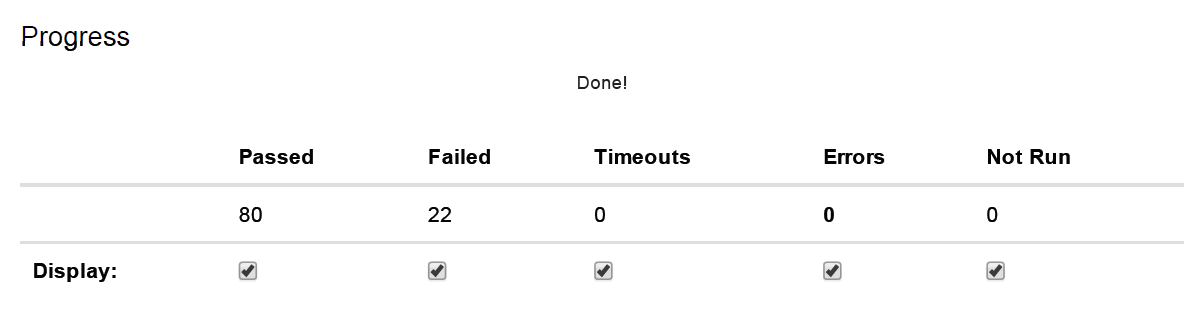
\includegraphics[width=6.5in]{img/test-results.png}
\end{figure*}

The tests were run using the regular approach the W3C recommends (see \href{https://github.com/w3c/web-platform-tests}{Web Platform Tests}) with the addition of priorly injecting the necessary scripts (see  \ref{scripts}) and defering the load of inline scripts running the actual tests by a nodejs script (see \href{https://github.com/ltetzlaff/inject-dependencies}{Github}.

Comparing this outcome with official implementation results the test compliance is on par with if not higher than CD53 from June 2016 \href{https://w3c.github.io/test-results/presentation-api/controlling-ua/all.html}{W3C Test results} with fails mostly eventuating from the above design decisions (see  \ref{architecture} and  \ref{shortcomings}) such as the necessity to construct a  {\lstinline[style=inline]$TrustedEvent$} which is reserved for the browser.

%\pagebreak
\newpage

\section{Demo}
\label{demo}
Included in the presentation is a simple controller page incorporating an embedded youtube video whose url is - upon connecting to a presentation display hosted in a separate site - transmitted to the Receiver and then loaded there as a Receiving Browsing Context. Furthermore certain click events in the controller document invoke a function call in the Receiving Browsing Context via a predefined micro-protocol to play and pause the video. Similar to the \href{https://google.com/chromecast}{Google Chromecast} Device a backdrop image and the display identification are displayed when the Controller is idle. The  \ref{configuration} handlers for e.g. the connection handshake or message exchange are implemented with a Node.JS app incorporating a hybrid approach of \href{https://socket.io}{Socket.io} and a more compatible ajax fallback.

To start it just hit  {\lstinline[style=inline]$npm start$} in  {\lstinline[style=inline]$%projectRoot%/server$} and send your browser to  {\lstinline[style=inline]$localhost:8080/receiver$} and  {\lstinline[style=inline]$localhost:8080/demo_video_controller$}.

\newpage
%\pagebreak
\section{Appendices}
\label{appendices}

The attached images show how the following usage looks like, after starting the display and thus the Receiver a backdrop image is visible. Loading the controlling application page instantiates the Controller. The user may now connect to a display of her choice after clicking the designated button. After the handshake is complete the url of the embedded video is exchanged and the user may toggle playback remotely. Similar to how Youtube on a Chromecast works other users may now enter the room (or the same user can reconnect if the presentationId is cached) and overwrite what is being shown on the display without revoking the right of the other participants to toggle video playback.


\begin{figure*}[!ht]
\centering\label{demo1}
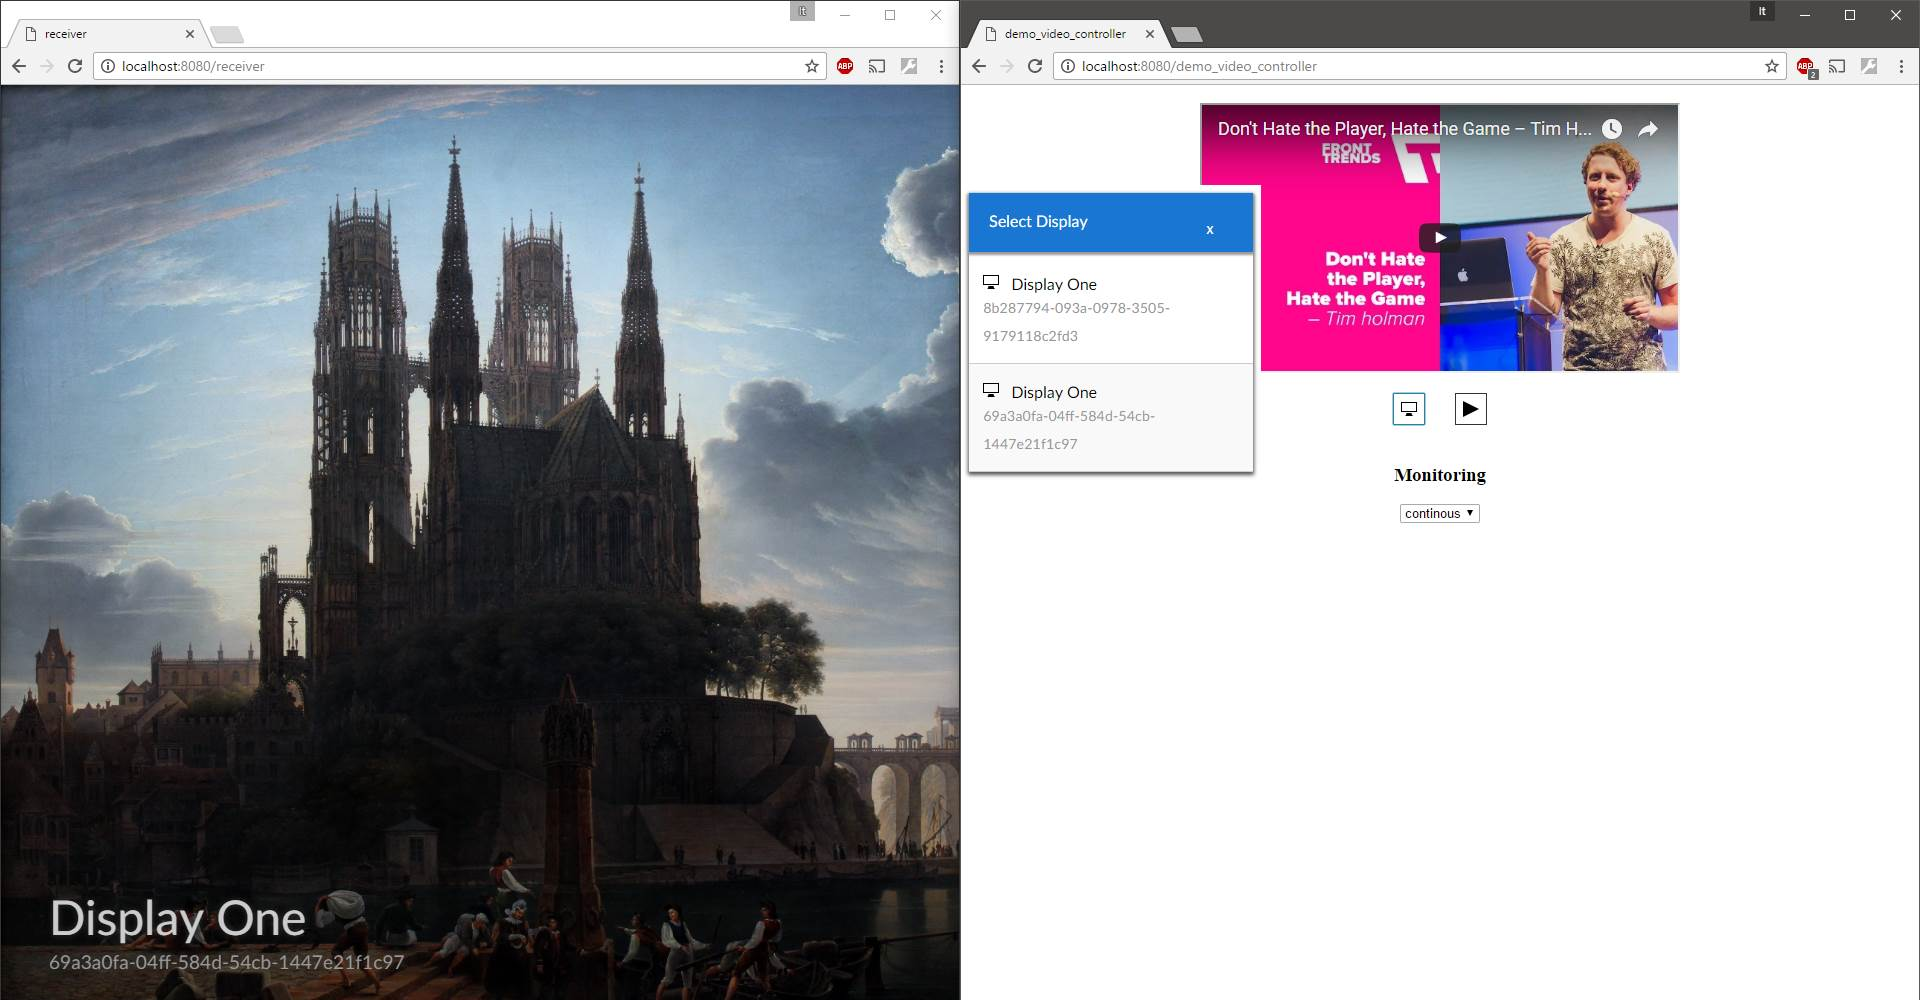
\includegraphics[width=6.5in]{img/demo1.jpg}
\end{figure*}

\begin{figure*}[!ht]
\centering\label{demo4}
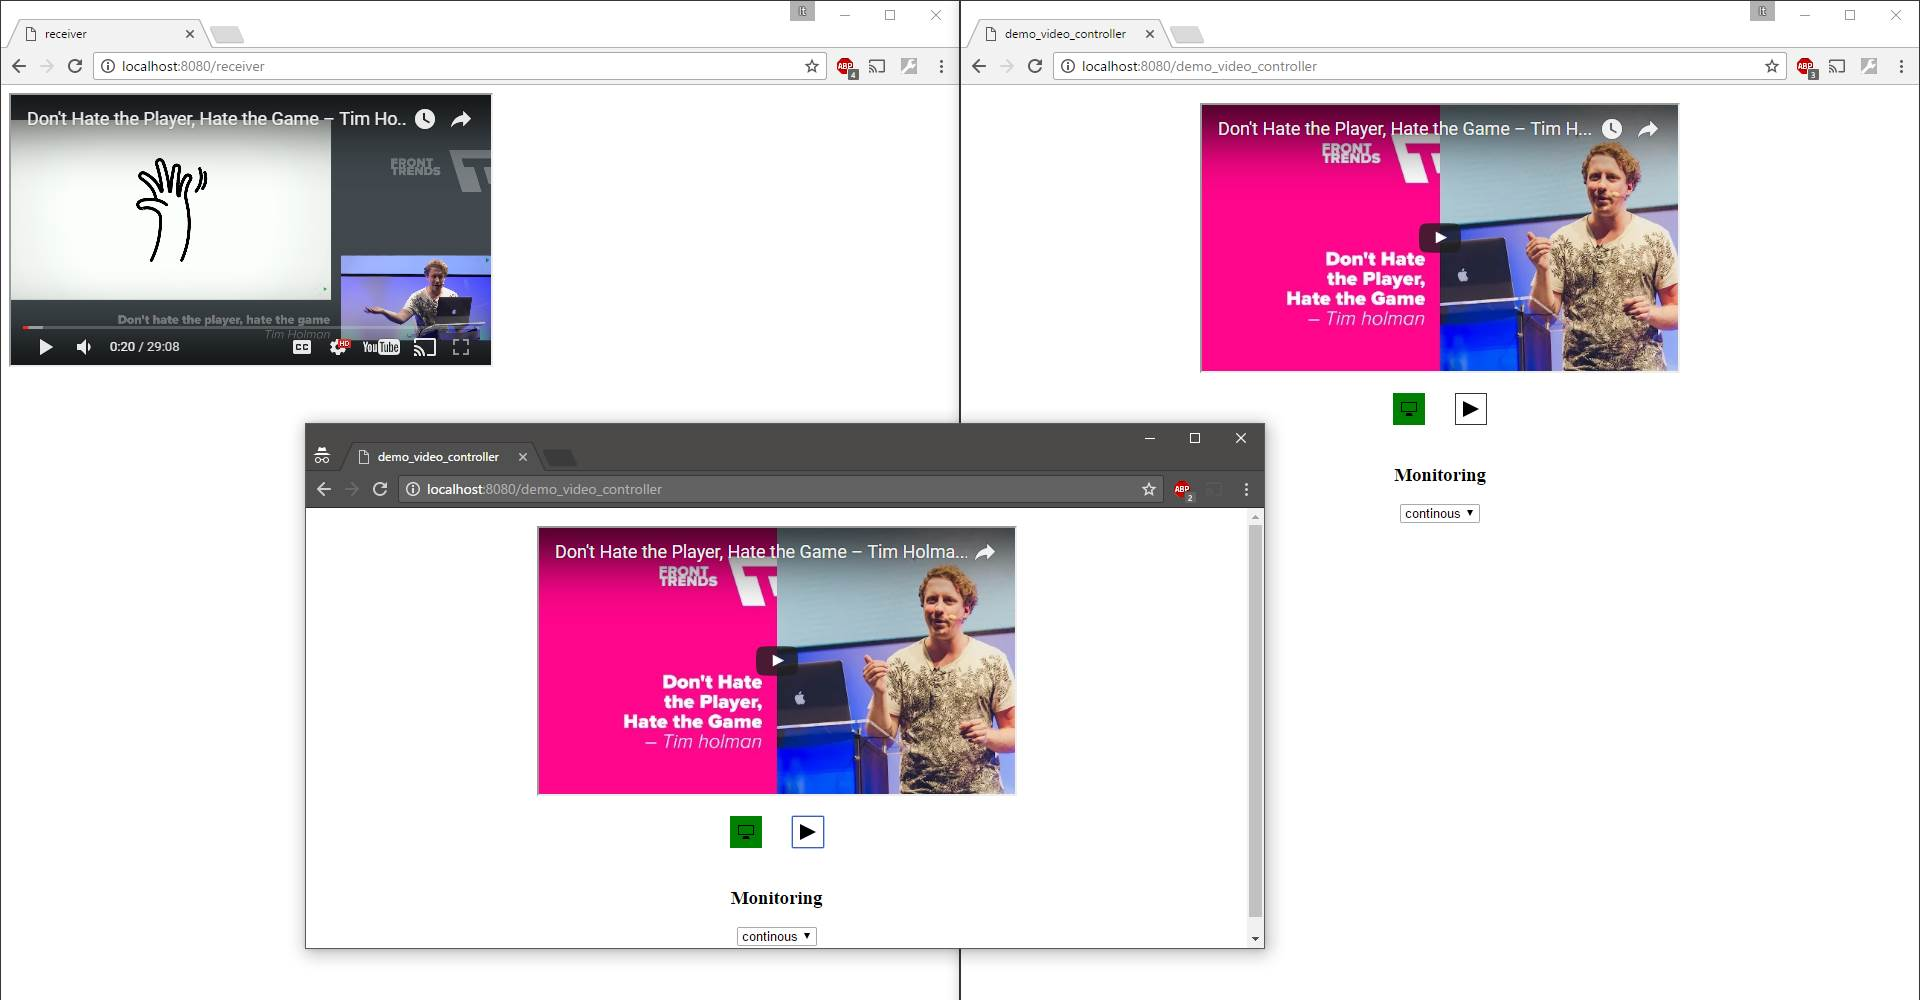
\includegraphics[width=6.5in]{img/demo4.jpg}
\end{figure*}

\begin{figure*}[!ht]
\centering
%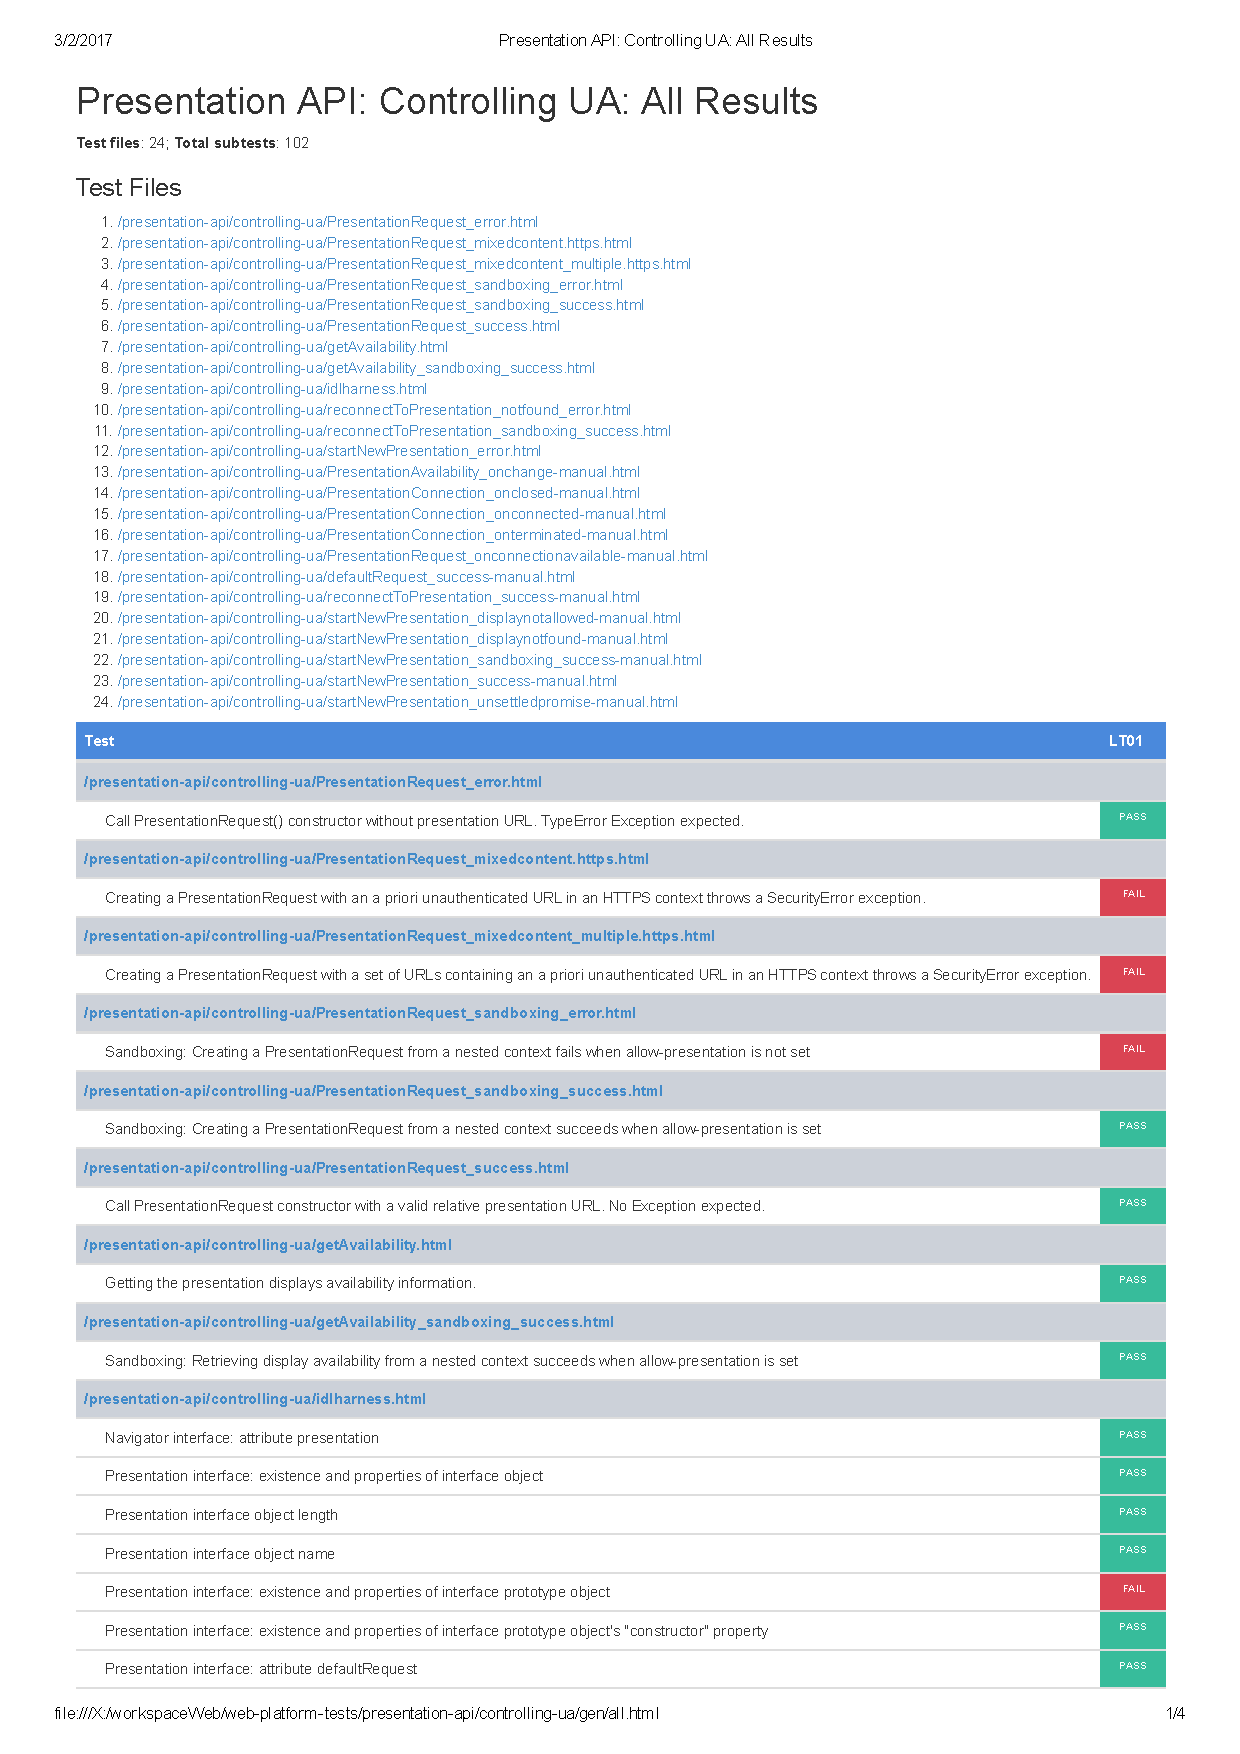
\includepdf[pages=-,width=.45\textwidth]{wptreport.pdf}
\begin{tabular}{@{}c@{\hspace{.5cm}}c@{}}
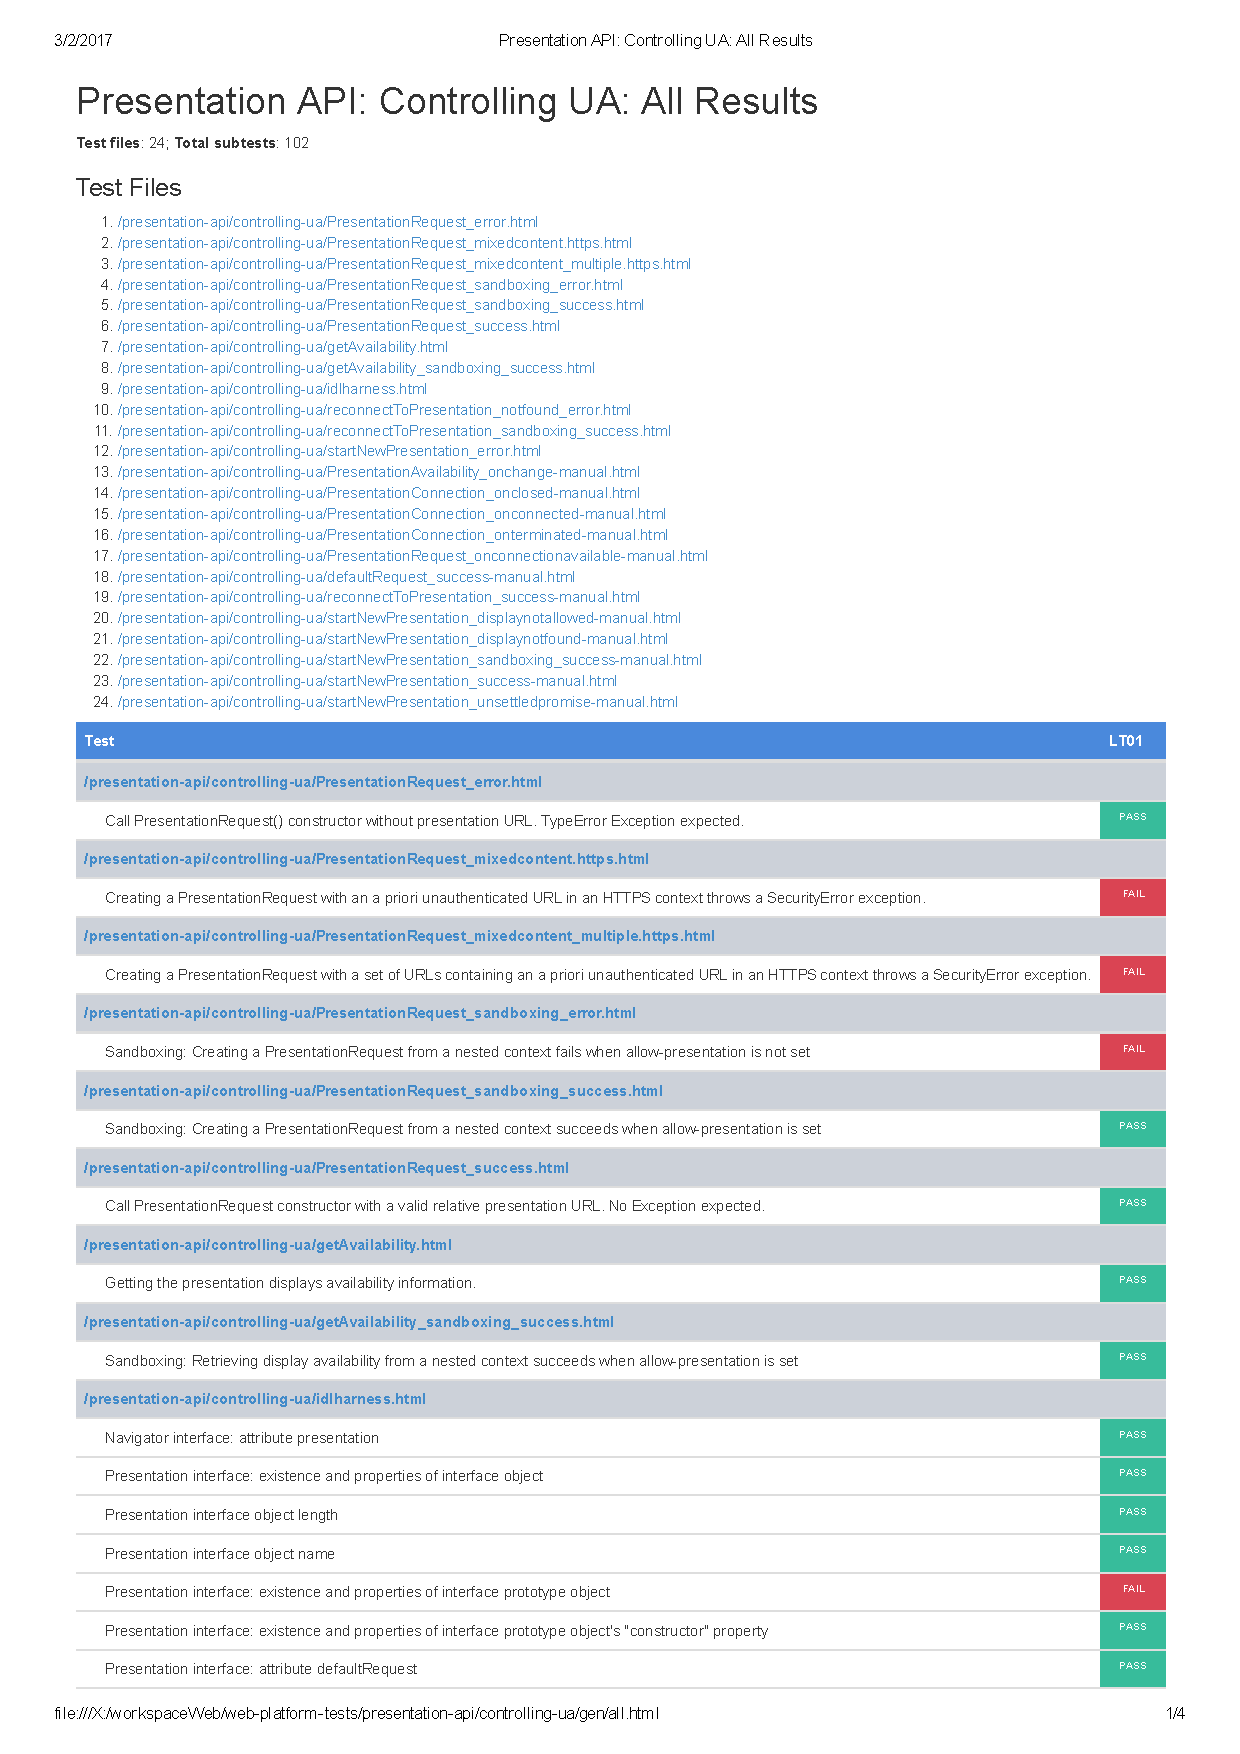
\includegraphics[page=1,width=.45\textwidth]{wptreport.pdf} & 
\includegraphics[page=2,width=.45\textwidth]{wptreport.pdf} \\[.5cm]
\includegraphics[page=3,width=.45\textwidth]{wptreport.pdf} &
\includegraphics[page=4,width=.45\textwidth]{wptreport.pdf} \\
\end{tabular}
\end{figure*}

\end{document}